% Auto-generated by figures/src/make_captions.py (numbers from figures/src/data). Usage:
% \begin{figure}[t]\centering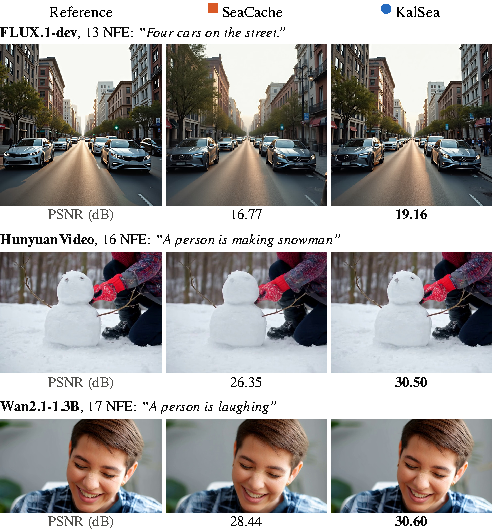
\includegraphics[width=\columnwidth]{figures/fig_qual_models.pdf}% Auto-generated by figures/src/make_captions.py (numbers from figures/src/data). Usage:
% \begin{figure}[t]\centering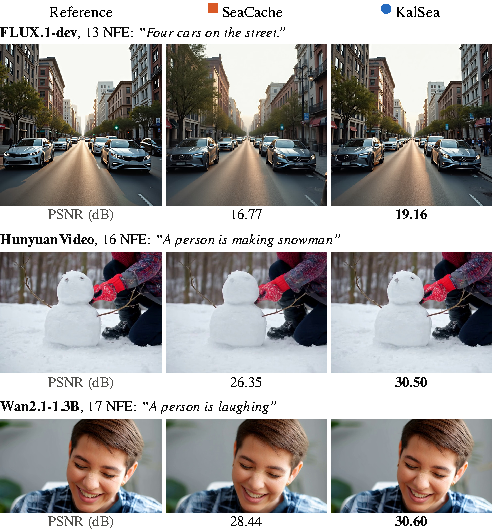
\includegraphics[width=\columnwidth]{figures/fig_qual_models.pdf}% Auto-generated by figures/src/make_captions.py (numbers from figures/src/data). Usage:
% \begin{figure}[t]\centering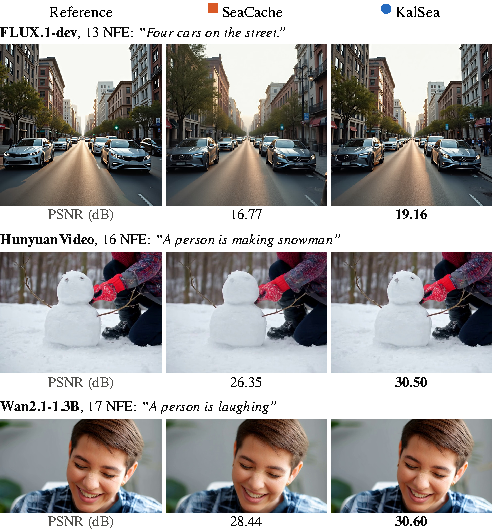
\includegraphics[width=\columnwidth]{figures/fig_qual_models.pdf}% Auto-generated by figures/src/make_captions.py (numbers from figures/src/data). Usage:
% \begin{figure}[t]\centering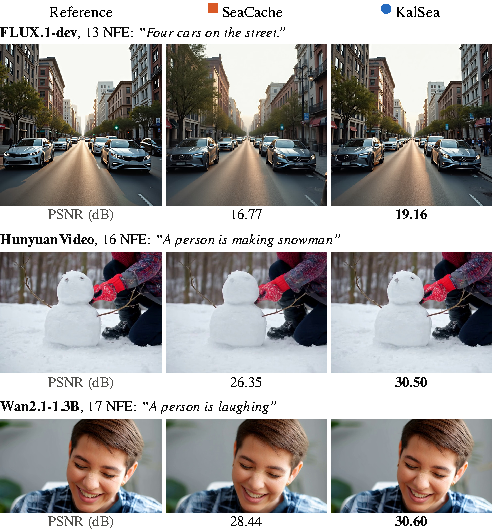
\includegraphics[width=\columnwidth]{figures/fig_qual_models.pdf}\input{figures/fig_qual_models_caption}\end{figure}
\caption{\textbf{One example per model at its lower budget}: \flux ($\delta=0.6$, 13 \nfe), HunyuanVideo ($\delta=0.48$, 16 \nfe, gate on the sampler's noise level), Wan2.1-1.3B ($\delta=0.35$, 17 \nfe); video: frame 32 of 65. Fixed rule: among the prompts on which \seacache and \ours computed identical steps, the one whose PSNR gain of \ours over \seacache is closest to the upper quartile. Numbers: per-image and per-video PSNR (dB) w.r.t.\ the 50-step reference. More in the supplement.}
\label{fig:qual-models}
\end{figure}
\caption{\textbf{One example per model at its lower budget}: \flux ($\delta=0.6$, 13 \nfe), HunyuanVideo ($\delta=0.48$, 16 \nfe, gate on the sampler's noise level), Wan2.1-1.3B ($\delta=0.35$, 17 \nfe); video: frame 32 of 65. Fixed rule: among the prompts on which \seacache and \ours computed identical steps, the one whose PSNR gain of \ours over \seacache is closest to the upper quartile. Numbers: per-image and per-video PSNR (dB) w.r.t.\ the 50-step reference. More in the supplement.}
\label{fig:qual-models}
\end{figure}
\caption{\textbf{One example per model at its lower budget}: \flux ($\delta=0.6$, 13 \nfe), HunyuanVideo ($\delta=0.48$, 16 \nfe, gate on the sampler's noise level), Wan2.1-1.3B ($\delta=0.35$, 17 \nfe); video: frame 32 of 65. Fixed rule: among the prompts on which \seacache and \ours computed identical steps, the one whose PSNR gain of \ours over \seacache is closest to the upper quartile. Numbers: per-image and per-video PSNR (dB) w.r.t.\ the 50-step reference. More in the supplement.}
\label{fig:qual-models}
\end{figure}
\caption{\textbf{One example per model at its lower budget}: \flux ($\delta=0.6$, 13 \nfe), HunyuanVideo ($\delta=0.48$, 16 \nfe, gate on the sampler's noise level), Wan2.1-1.3B ($\delta=0.35$, 17 \nfe); video: frame 32 of 65. Fixed rule: among the prompts on which \seacache and \ours computed identical steps, the one whose PSNR gain of \ours over \seacache is closest to the upper quartile. Numbers: per-image and per-video PSNR (dB) w.r.t.\ the 50-step reference. More in the supplement.}
\label{fig:qual-models}
